%!TEX root = ../dissertation.tex

% =====================================================================
%  APPENDIX B — Qualitative panels & query-text failure analysis
% ---------------------------------------------------------------------
%  Numbers computed by the text-pattern analysis cell in
%  notebooks/final_experimental_results.ipynb (Ours_J/p_context pipeline,
%  full i-CIR, 1,883 queries). Global mean AP = 39.77%, fail rate = 24.9%
%  (AP < 10%). Only tokens appearing in ≥ 8 queries are included.
%  Enrichment = per-token fail rate / global fail rate (>1 = overrepresented).
% =====================================================================

\chapter{Qualitative Panels and Failure-Pattern Analysis}\label{app:qual_analysis}

This appendix provides additional qualitative retrieval panels and a
token-level statistical analysis of failure patterns in the \emph{Ours}
pipeline (CLIP-L, INSTR\,J, \texttt{+context} rung).

% ---------------------------------------------------------------------
\section*{Additional Success Panels}

The panels below show further queries where the triplet (\emph{Ours}) succeeds
while the duplet baselines (\textsc{Img}$\times$\textsc{Txt} and
\textsc{Basic}) fail. Each row corresponds to one method; correct retrievals
are bordered in green, incorrect in red.

\begin{figure}[htbp]
\centering
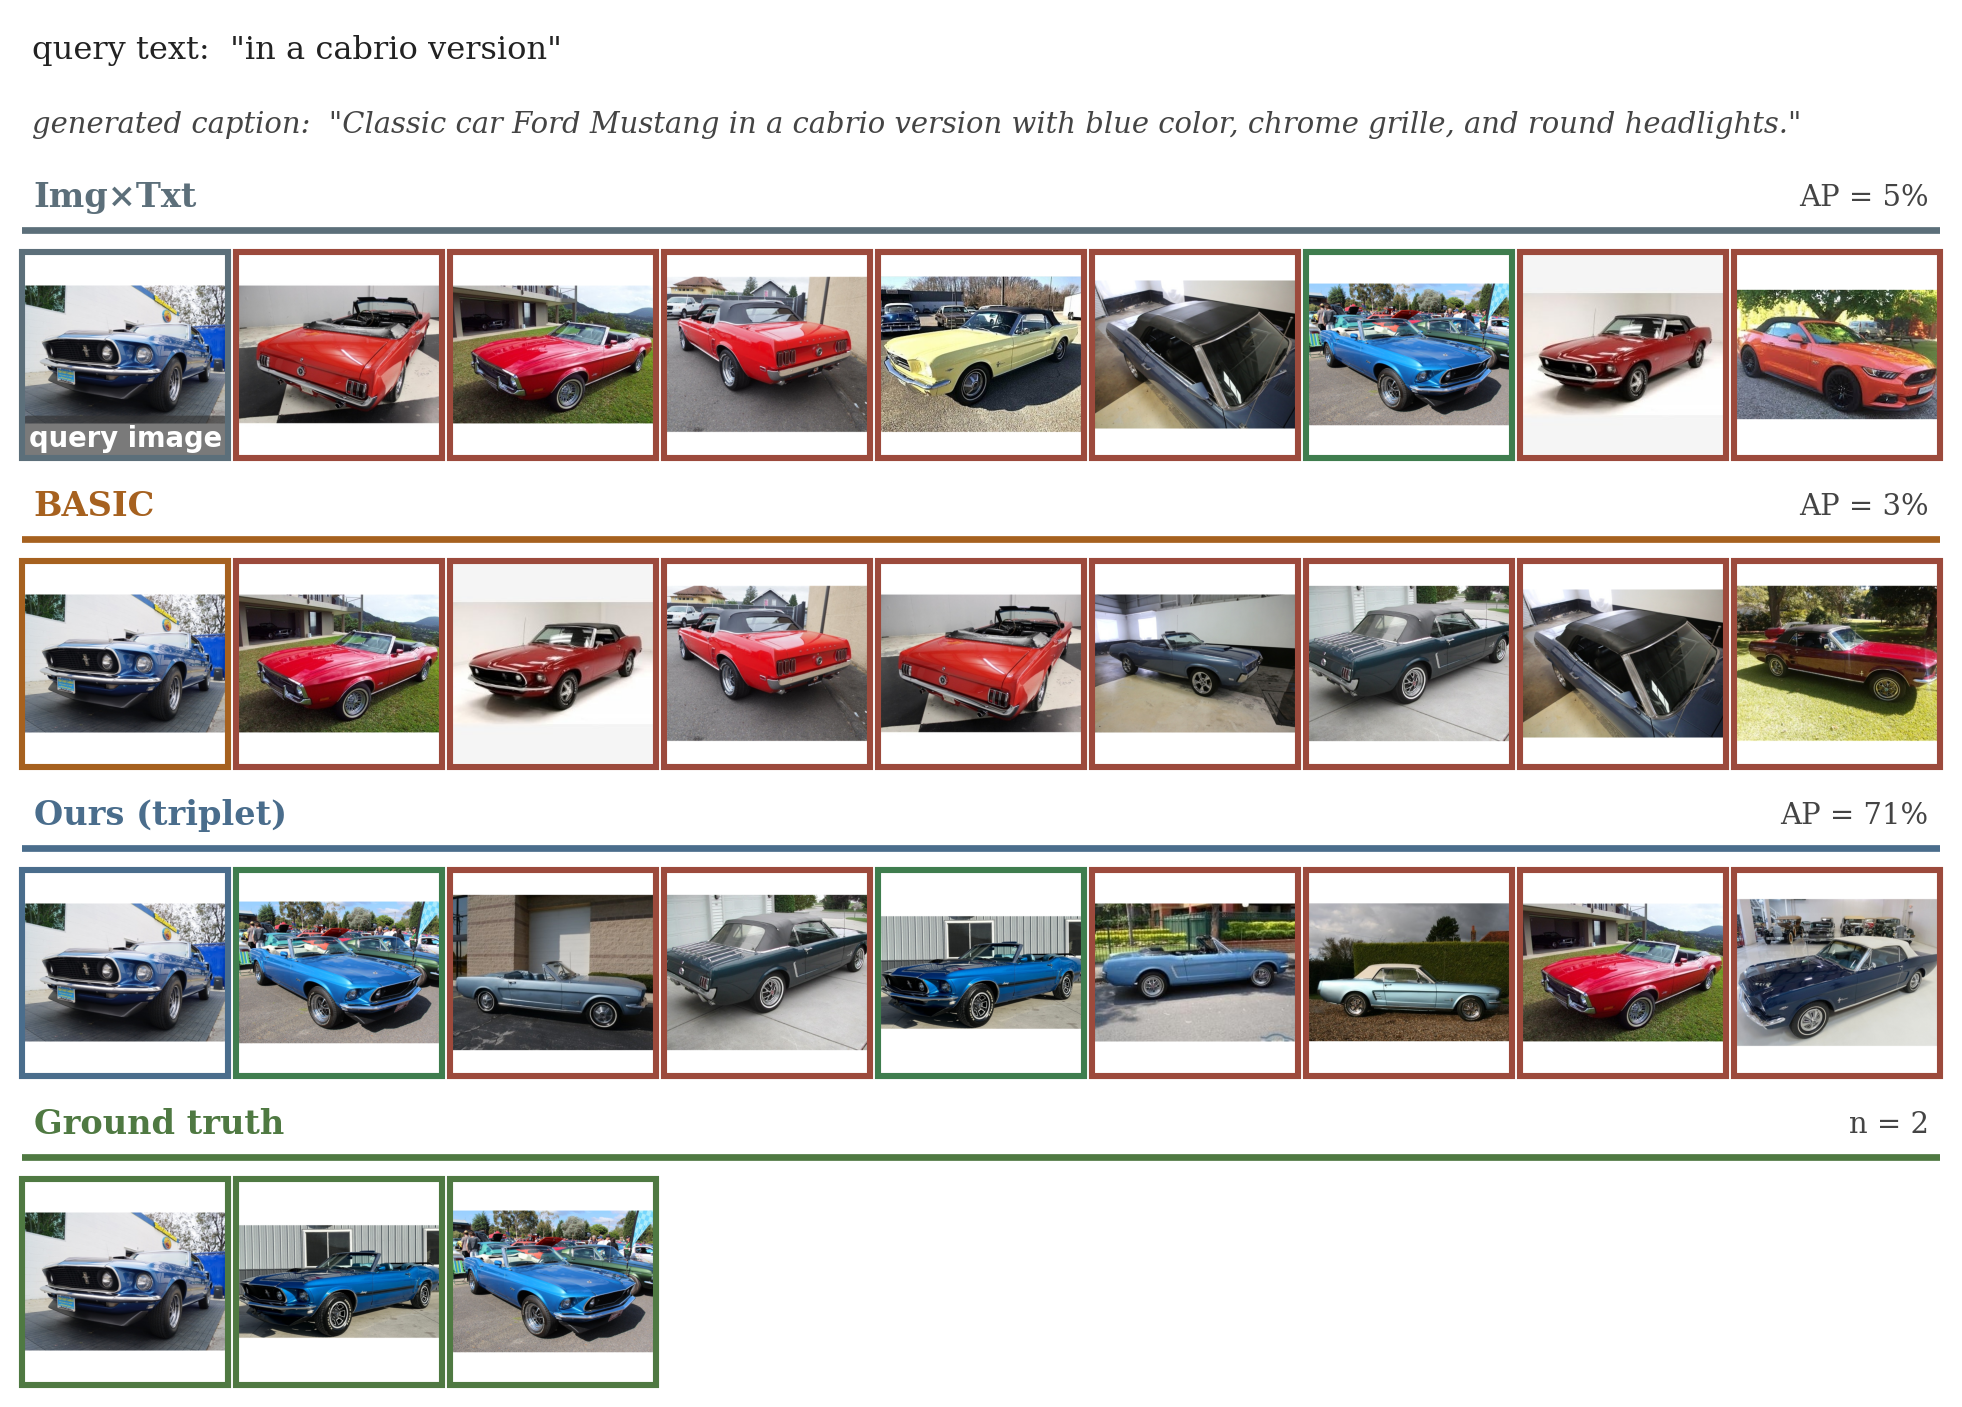
\includegraphics[width=\textwidth]{figures/qualitative_success_q682.png}
\end{figure}
\begin{figure}[htbp]
\centering
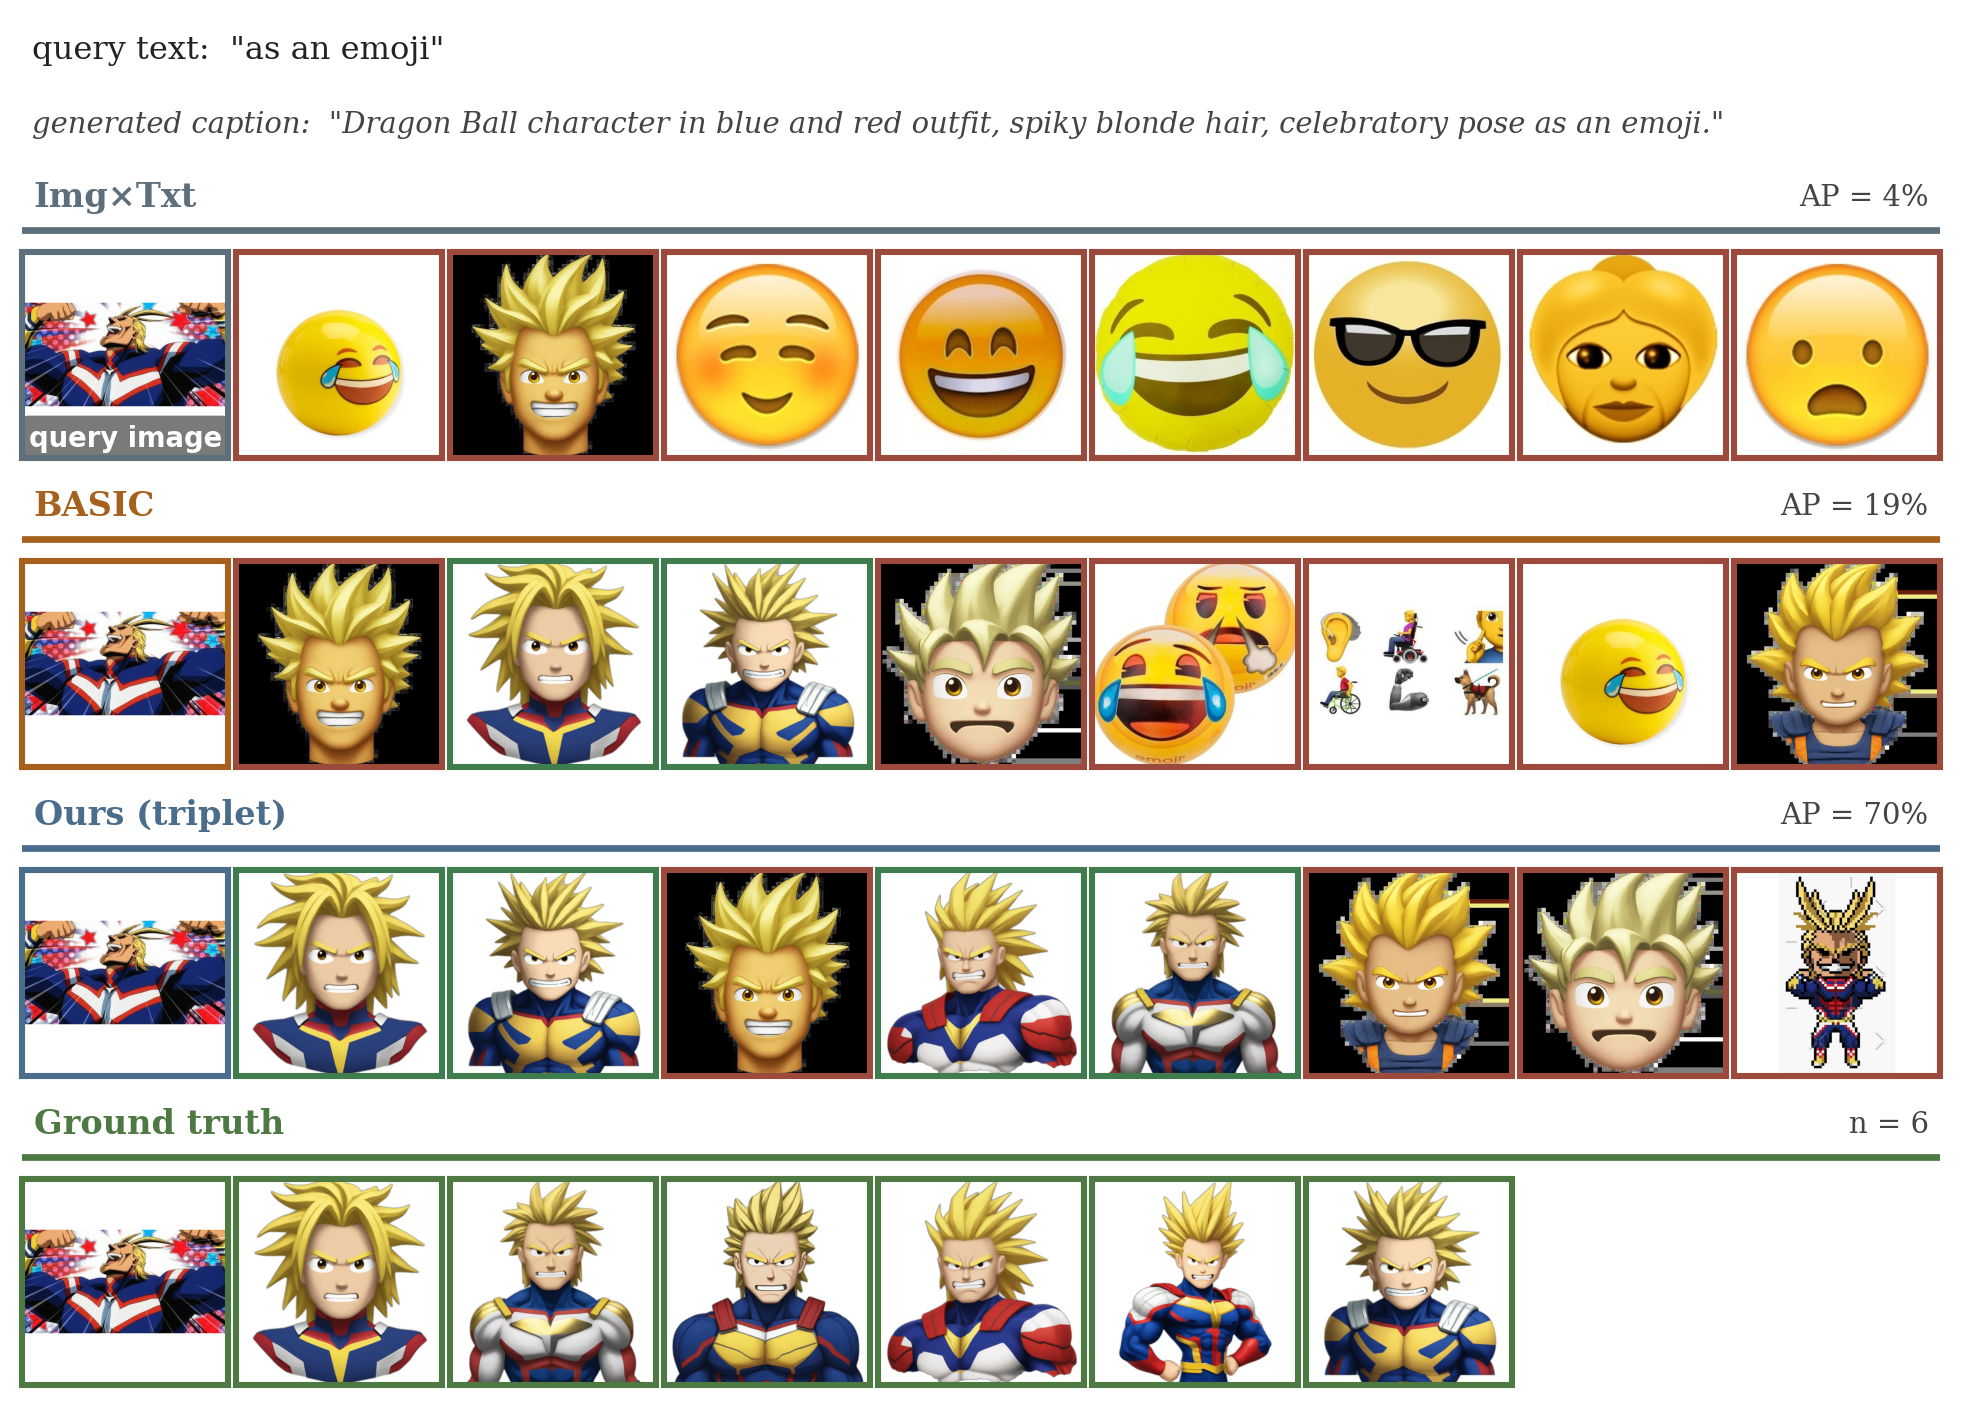
\includegraphics[width=\textwidth]{figures/qualitative_success_q48.png}
\end{figure}
\begin{figure}[htbp]
\centering
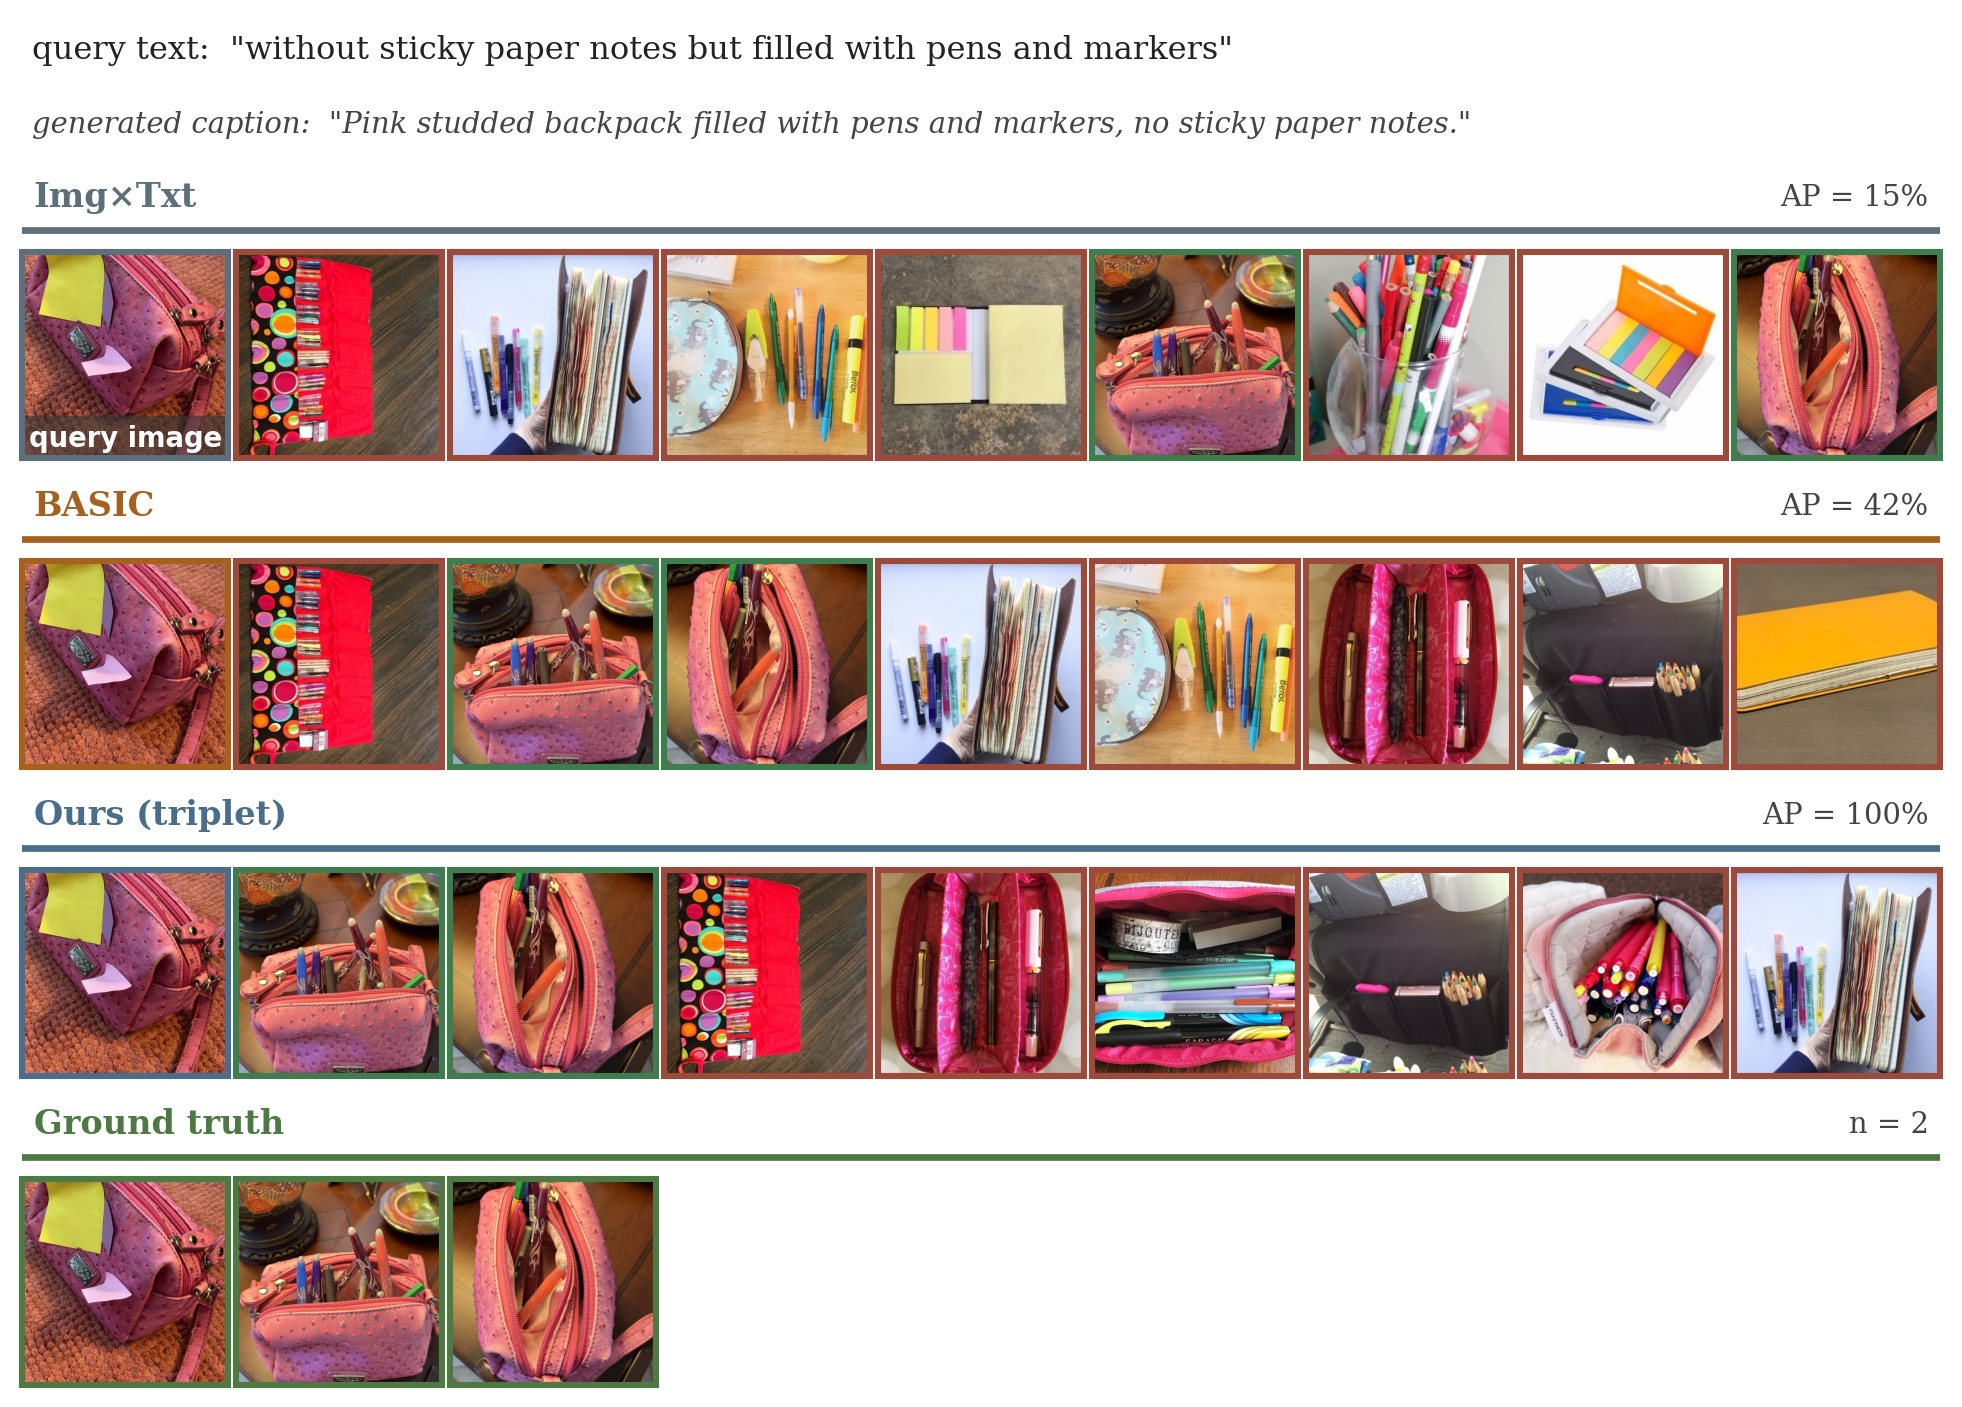
\includegraphics[width=\textwidth]{figures/qualitative_success_q1381.png}
\end{figure}

% ---------------------------------------------------------------------
\section*{Additional Failure Panels}

\begin{figure}[htbp]
\centering
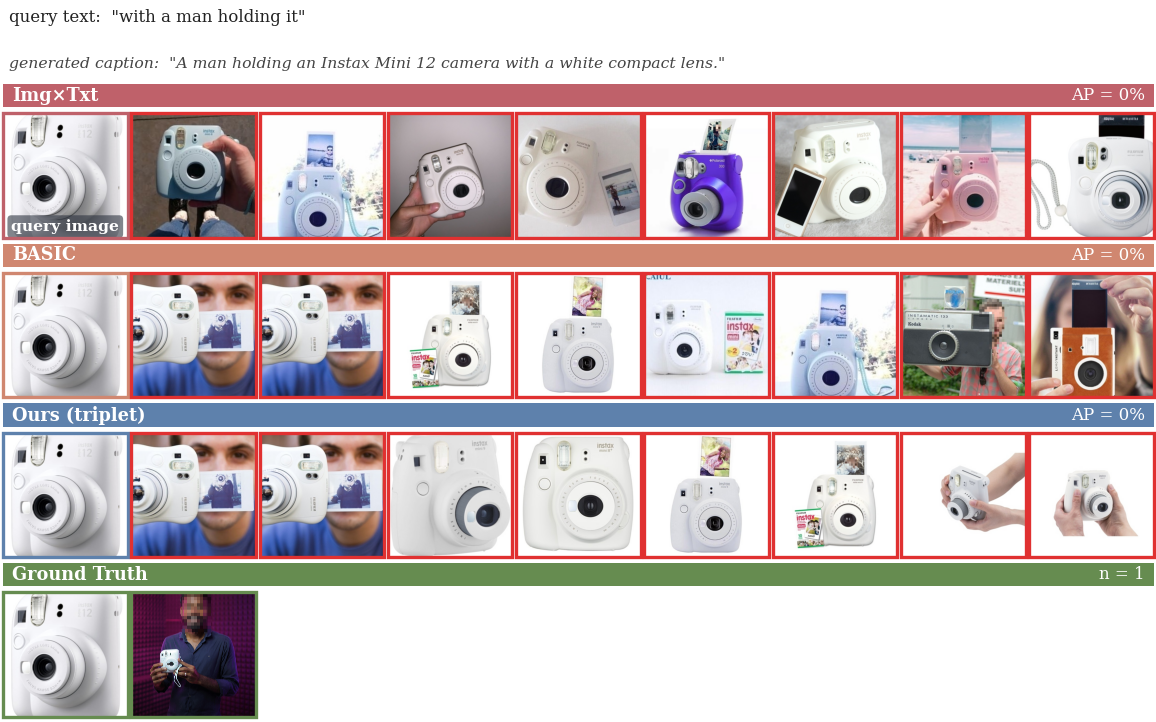
\includegraphics[width=\textwidth]{figures/qualitative_failure_q696.png}
\end{figure}
\begin{figure}[htbp]
\centering
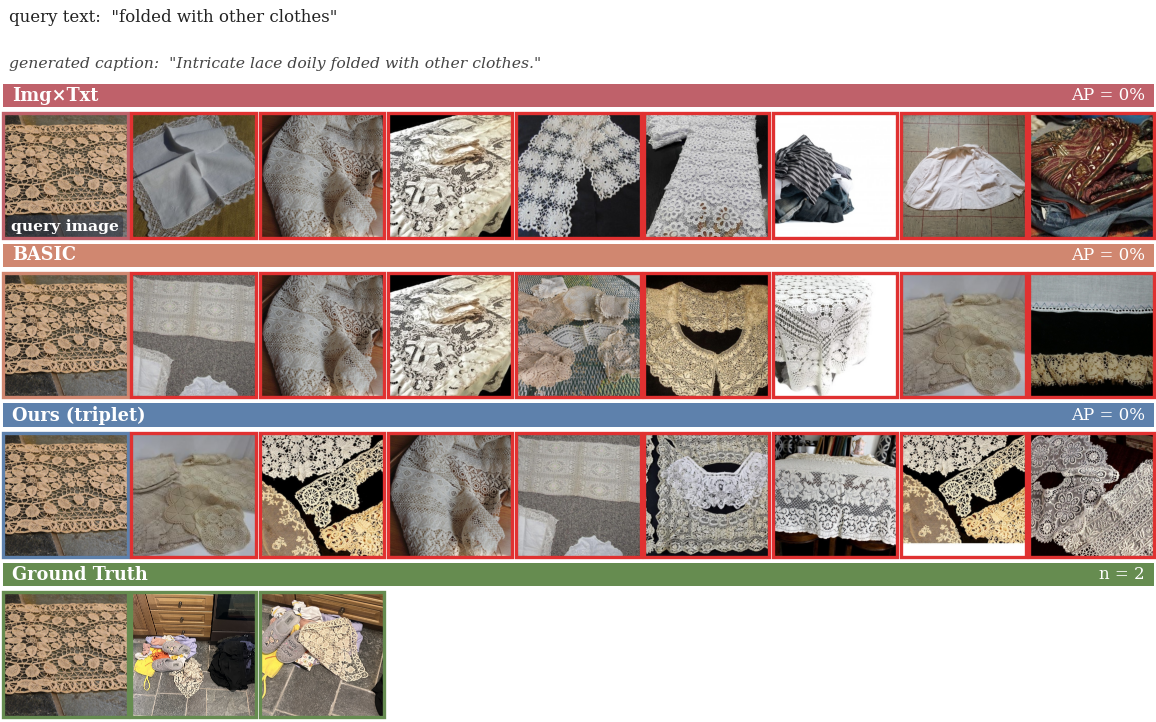
\includegraphics[width=\textwidth]{figures/qualitative_failure_q529.png}
\end{figure}
\begin{figure}[htbp]
\centering
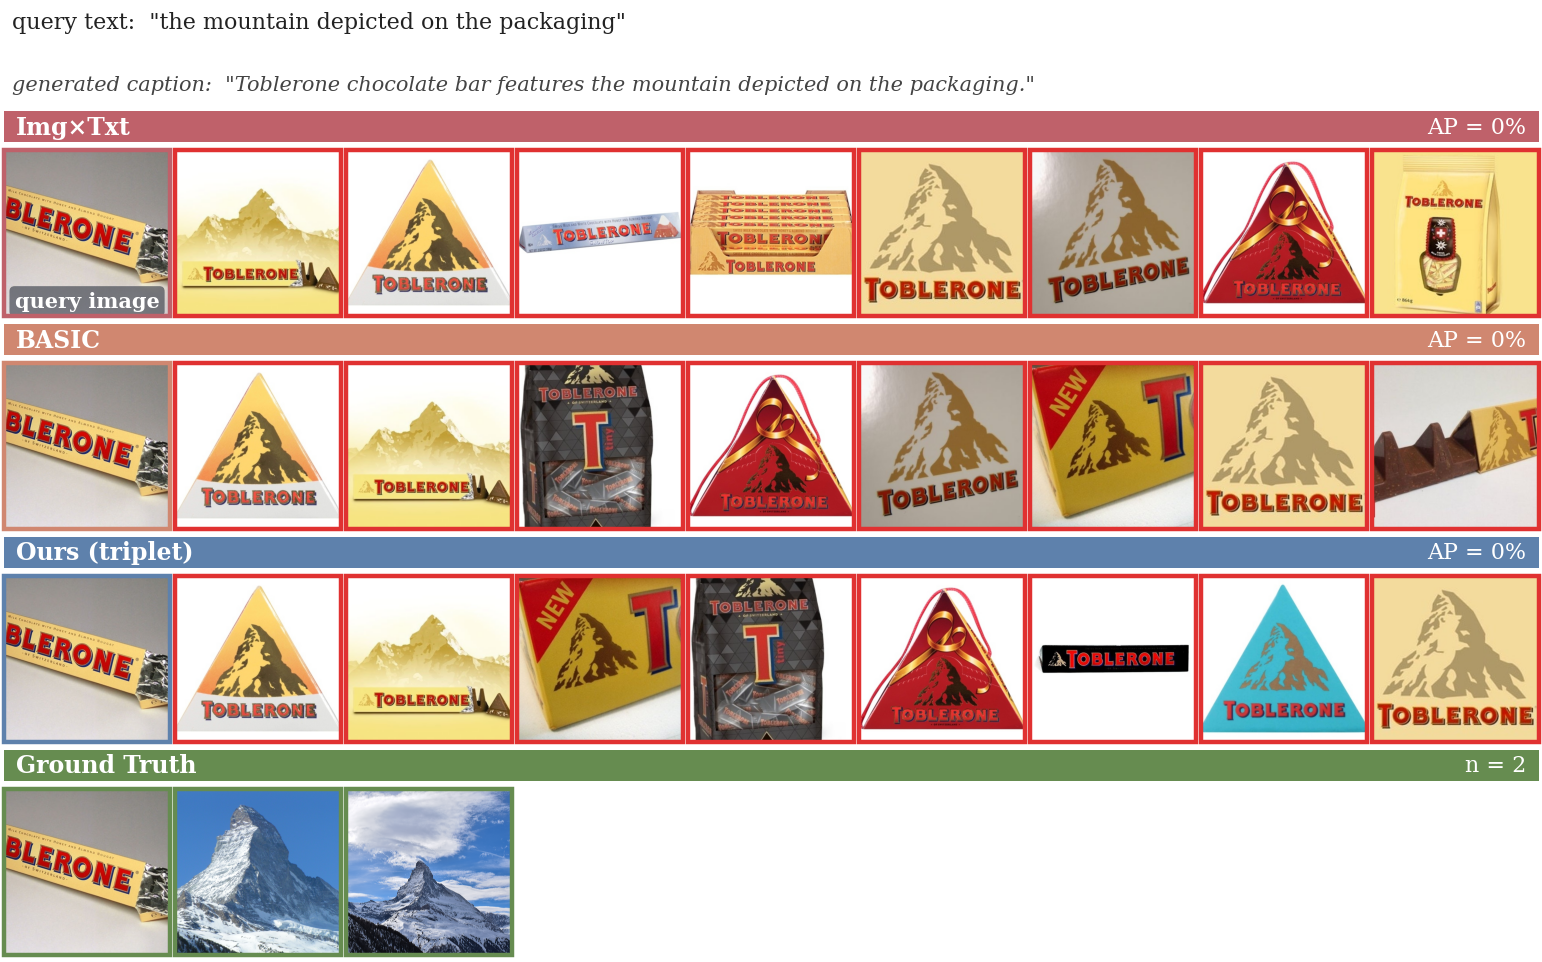
\includegraphics[width=\textwidth]{figures/qualitative_failure_q1785.png}
\end{figure}
\begin{figure}[htbp]
\centering
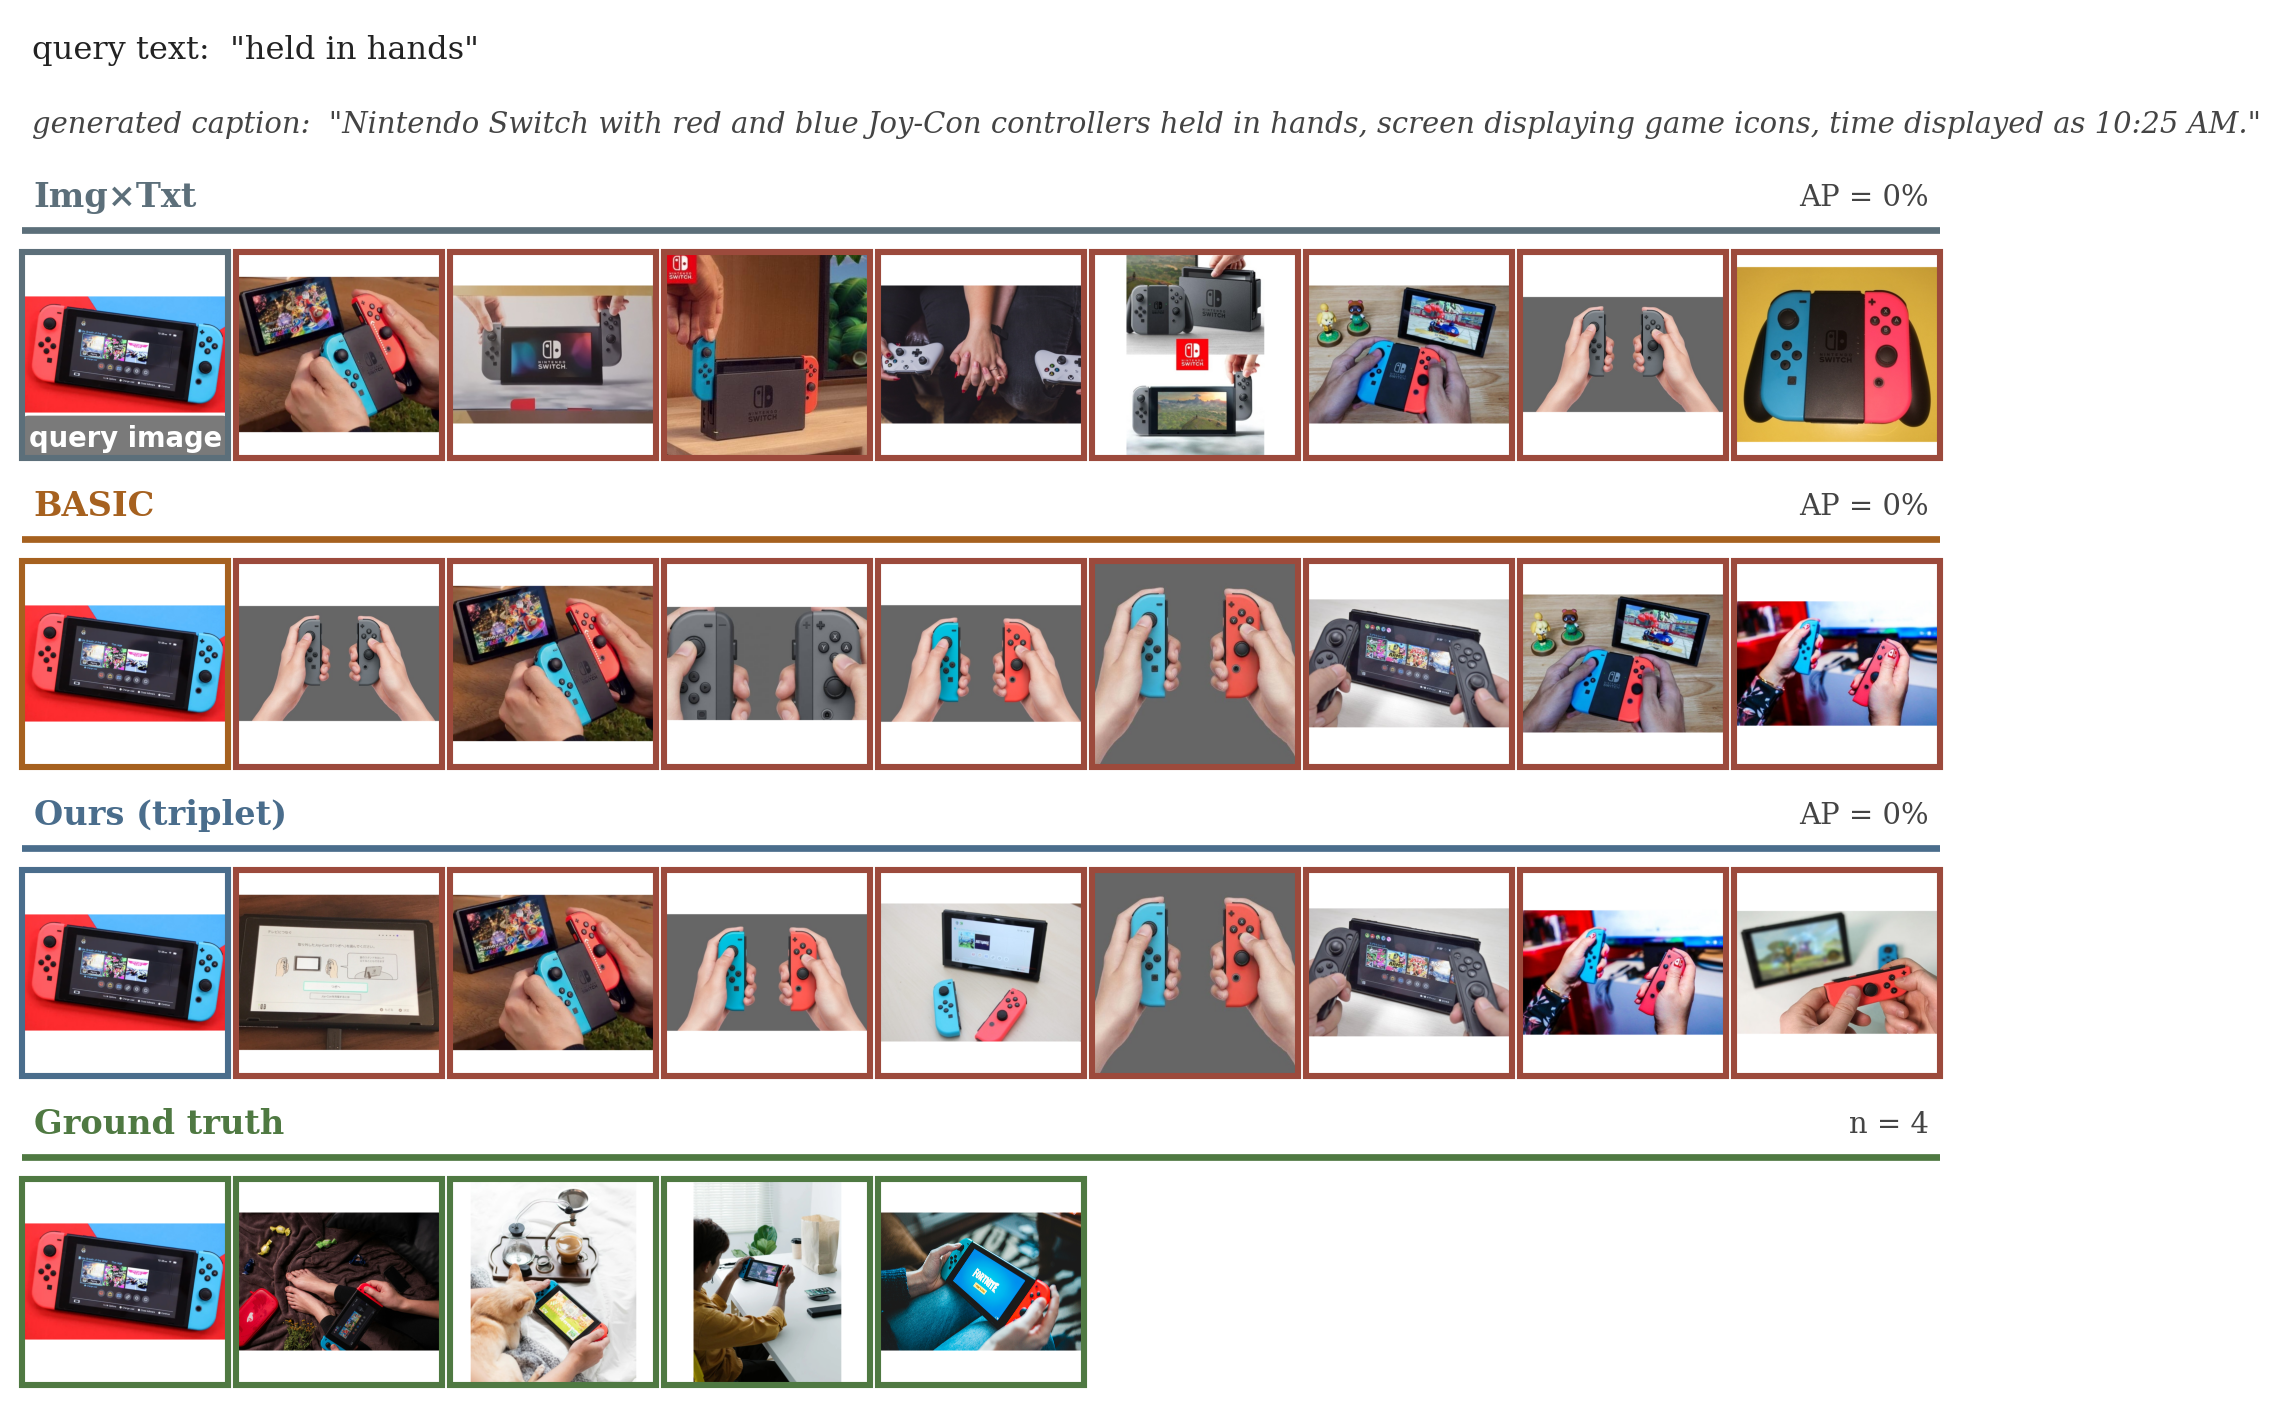
\includegraphics[width=\textwidth]{figures/qualitative_failure_q1260.png}
\end{figure}

% ---------------------------------------------------------------------
\section*{Query-Text Failure-Pattern Analysis}

To identify linguistic patterns that systematically correlate with low
retrieval performance, we tokenise each of the 1,883 modification texts
(lowercased, stopwords removed) into unigrams and bigrams and compute,
for each token appearing in at least eight queries: mean per-query AP,
failure rate (AP\,$<10\%$), and \emph{enrichment} (per-token failure
rate divided by the global failure rate of $24.9\%$).  Enrichment
$>1$ indicates the token is overrepresented in failed queries.

Table~\ref{tab:app_worst_tokens} lists the 15 tokens with the lowest
mean AP; Table~\ref{tab:app_best_tokens} lists the 10 tokens with the
highest mean AP. Together they reveal a sharp contrast: highly distinctive,
nameable targets (\textit{lego}, \textit{fog}, \textit{sweater},
\textit{balloon}) achieve near-zero failure rates, while modifications
requesting out-of-distribution states or contexts (\textit{worn},
\textit{folded}, \textit{food}, \textit{film}) cluster at high failure rates
regardless of caption quality.

\begin{table}[htbp]
\centering
\caption{Tokens most enriched in failed queries (AP\,$<\!10\%$), sorted by
mean AP. Enrichment $= $ per-token fail rate\,/\,global fail rate ($24.9\%$).
Minimum 8 queries per token.}
\label{tab:app_worst_tokens}
\small
\begin{tabular}{l r r r r}
\toprule
Modification term & $n$ & Mean AP (\%) & Fail rate (\%) & Enrichment \\
\midrule
original              &  8 &  1.4 & 100.0 & 4.0 \\
food                  & 10 &  1.6 & 100.0 & 4.0 \\
worn                  & 23 &  2.7 &  91.3 & 3.7 \\
film                  &  9 &  2.8 & 100.0 & 4.0 \\
table                 & 11 &  3.1 &  90.9 & 3.6 \\
folded                &  9 &  4.4 &  88.9 & 3.6 \\
dog                   & 12 &  5.0 &  75.0 & 3.0 \\
dark                  & 10 &  6.7 &  80.0 & 3.2 \\
leather               & 10 &  6.7 &  80.0 & 3.2 \\
beige                 & 10 &  6.7 &  80.0 & 3.2 \\
holder                &  8 &  7.8 &  87.5 & 3.5 \\
case                  & 11 &  8.4 &  63.6 & 2.6 \\
other                 & 15 &  9.5 &  73.3 & 2.9 \\
real size             & 14 & 11.0 &  64.3 & 2.6 \\
monochrome engraving  & 26 & 11.9 &  57.7 & 2.3 \\
\bottomrule
\end{tabular}
\end{table}

\begin{table}[htbp]
\centering
\caption{Tokens with the highest mean AP (\emph{Ours}), sorted
descending. Win rate = fraction of queries with AP\,$\ge\!50\%$.}
\label{tab:app_best_tokens}
\small
\begin{tabular}{l r r r}
\toprule
Modification term & $n$ & Mean AP (\%) & Win rate (\%) \\
\midrule
watercolor painting &  8 & 87.5 & 100.0 \\
fog                 & 27 & 86.1 &  92.6 \\
lego                & 35 & 85.7 &  88.6 \\
sweater             &  8 & 84.0 & 100.0 \\
lego brick          &  9 & 80.2 & 100.0 \\
huge balloon        & 24 & 73.4 &  83.3 \\
watercolor          & 10 & 70.1 &  80.0 \\
aerial perspective  & 20 & 67.3 &  80.0 \\
figurine            & 12 & 66.5 &  66.7 \\
huge                & 31 & 65.3 &  71.0 \\
\bottomrule
\end{tabular}
\end{table}

\subsection*{Lowest-AP Queries}

Table~\ref{tab:app_bottom_queries} lists the 30 queries with the lowest
\emph{Ours} AP, together with the full modification text.  Three
modification phrasings account for the majority: ``being deflated''
(instances that simply have no deflated counterpart in the database),
``as a painting'' (domain transfer with no database coverage), and
``worn by a dog'' / ``worn by a person'' / ``worn on the ankle''
(context-breaking wearable modifications).

\begin{table}[htbp]
\centering
\caption{Bottom-30 queries by \emph{Ours} AP (Ours\,[\textsc{J}],
\texttt{+context}, full i-CIR).}
\label{tab:app_bottom_queries}
\small
\begin{tabular}{r r l}
\toprule
Query ID & AP (\%) & Modification text \\
\midrule
 861 & 0.0 & being deflated \\
 869 & 0.1 & being deflated \\
1100 & 0.1 & as a painting \\
1496 & 0.1 & worn by a dog \\
 529 & 0.1 & folded with other clothes \\
1490 & 0.1 & worn by a dog \\
1096 & 0.1 & as a painting \\
 865 & 0.1 & being deflated \\
1104 & 0.1 & as a painting \\
1356 & 0.1 & as a photo during day \\
1493 & 0.1 & worn by a dog \\
1354 & 0.1 & as a photo during day \\
1652 & 0.1 & worn by a person \\
1785 & 0.1 & the mountain depicted on the packaging \\
 662 & 0.1 & folded \\
1098 & 0.1 & as a painting \\
1102 & 0.1 & as a painting \\
1649 & 0.1 & worn by a person \\
1825 & 0.1 & on a bookshelf \\
1819 & 0.1 & stored in a wardrobe \\
1826 & 0.1 & lying open \\
1646 & 0.1 & worn by a person \\
1383 & 0.1 & worn around a dog's neck \\
 416 & 0.1 & worn on the ankle \\
1821 & 0.2 & worn \\
 106 & 0.2 & with various ornaments displayed on top \\
 103 & 0.2 & with various ornaments displayed on top \\
1495 & 0.2 & worn on a face sculpture \\
 696 & 0.2 & with a man holding it \\
1489 & 0.2 & worn on a face sculpture \\
\bottomrule
\end{tabular}
\end{table}
